\newpage
\section{3次元スロッシング}

\subsection{解析条件}

水平加速度$f_{x}$は以下の式で与える。
\begin{equation}
	f_{x} = A \omega^2 \sin{\omega t}
\end{equation}
ここで、振幅$A=0.0093 \mathrm{m}$、角速度$\omega = 5.311 \mathrm{rad/s}$である。

\renewcommand{\arraystretch}{1}
\begin{table}[H]
	\centering
	\caption{物性値}
	\begin{tabular}{ccccccc}
		\hline
		Test case & $\rho_1$ & $\rho_2$ & $\mu_1$ & $\mu_2$ & $\mathrm{g}$ \\
		\hline 
		Case$1$ & $1000$ & $100$ & $10$ & $1$   & $0.98$ \\
		\hline         
	\end{tabular}
	\label{table:3d-bubble-material-property}
\end{table}
\renewcommand{\arraystretch}{1.0}

\renewcommand{\arraystretch}{1}
\begin{table}[H]
	\centering
	\caption{解析パラメータ}
	\begin{tabular}{cccccc}
		\hline
		Test case & $\Delta t$ & メッシュ幅$dx$ & 界面幅$D$ & 再初期化回数 & 再初期化$\Delta \tau$\\
		\hline 
		Case$1$ & $0.0025$ & $0.05$ & $0.04$ & $5$ & $0.0001$\\
		\hline         
	\end{tabular}
	\label{table:3d-bubble-parameter}
\end{table}
\renewcommand{\arraystretch}{1.0}

メッシュは六面体1次要素で、節点数18,081、要素数15,360である。

\begin{figure}[H]
	\centering
	\begin{minipage}[b]{0.49\columnwidth}
	    \centering
	    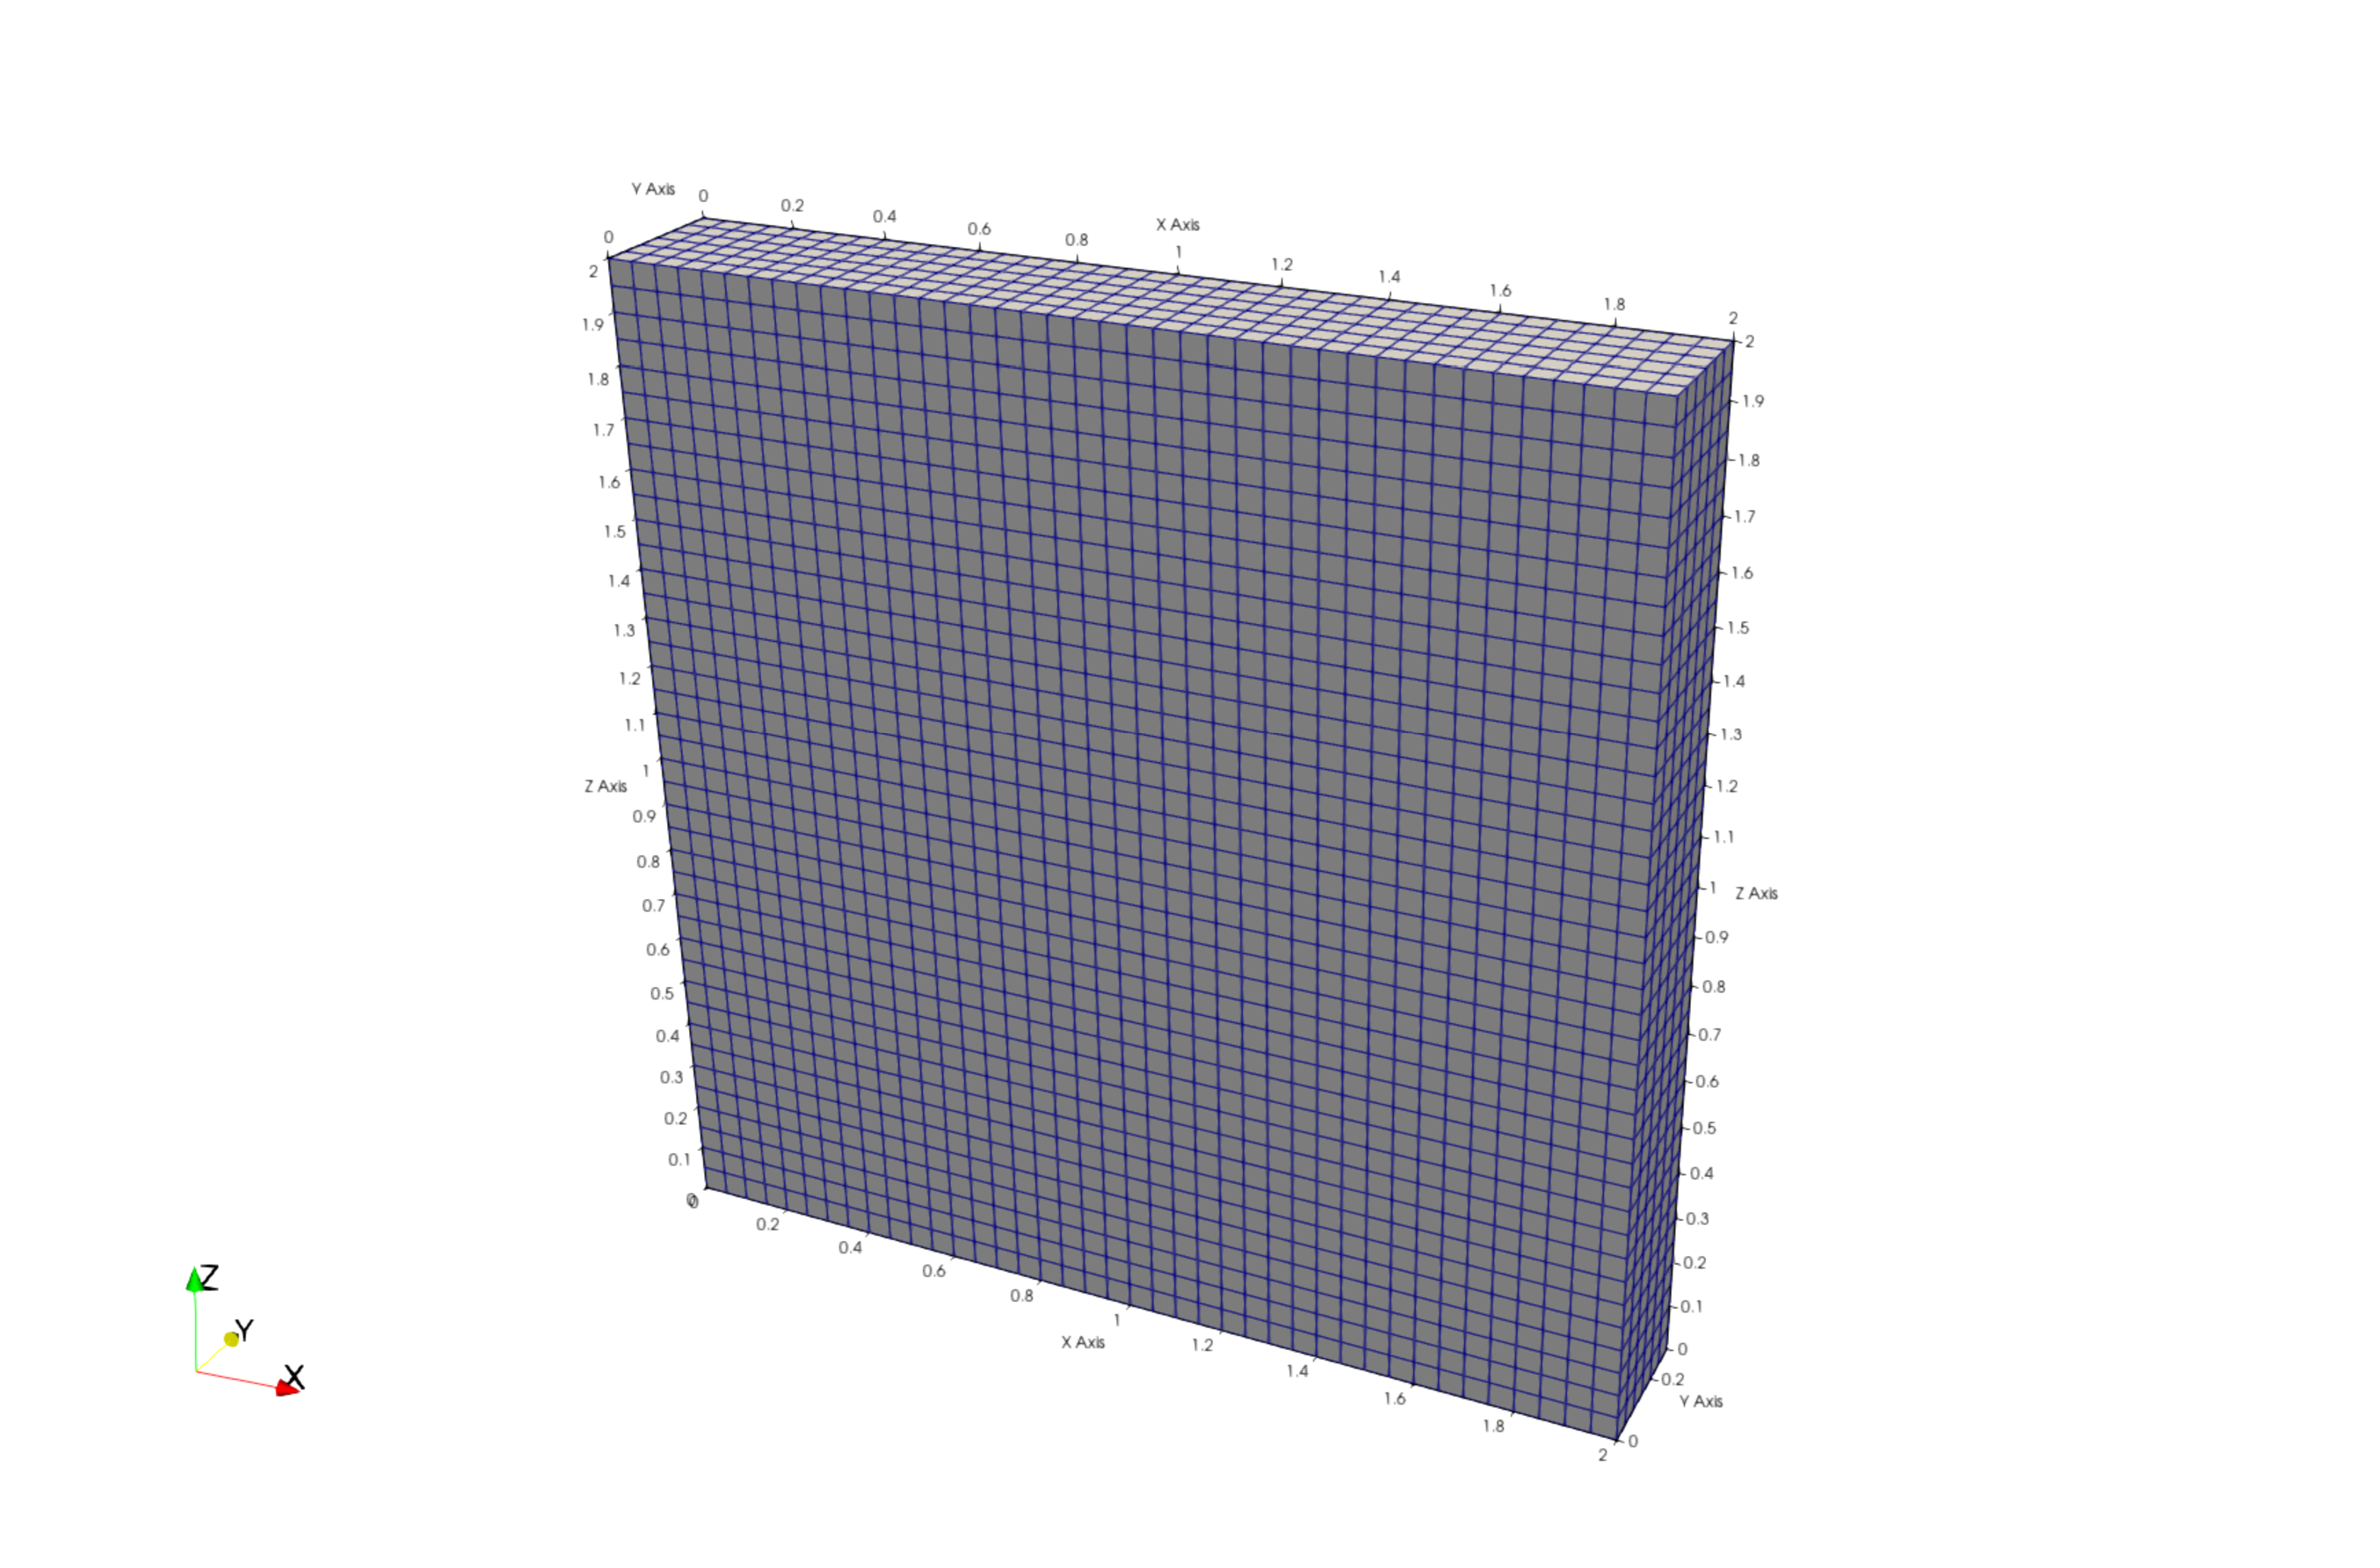
\includegraphics[width=6truecm]{pics/3d-sloshing/mesh.jpeg}
		\caption{3次元スロッシングの計算メッシュ}
		\label{fig:3d-sloshing-mesh}
	\end{minipage}
	\begin{minipage}[b]{0.49\columnwidth}
	    \centering
	    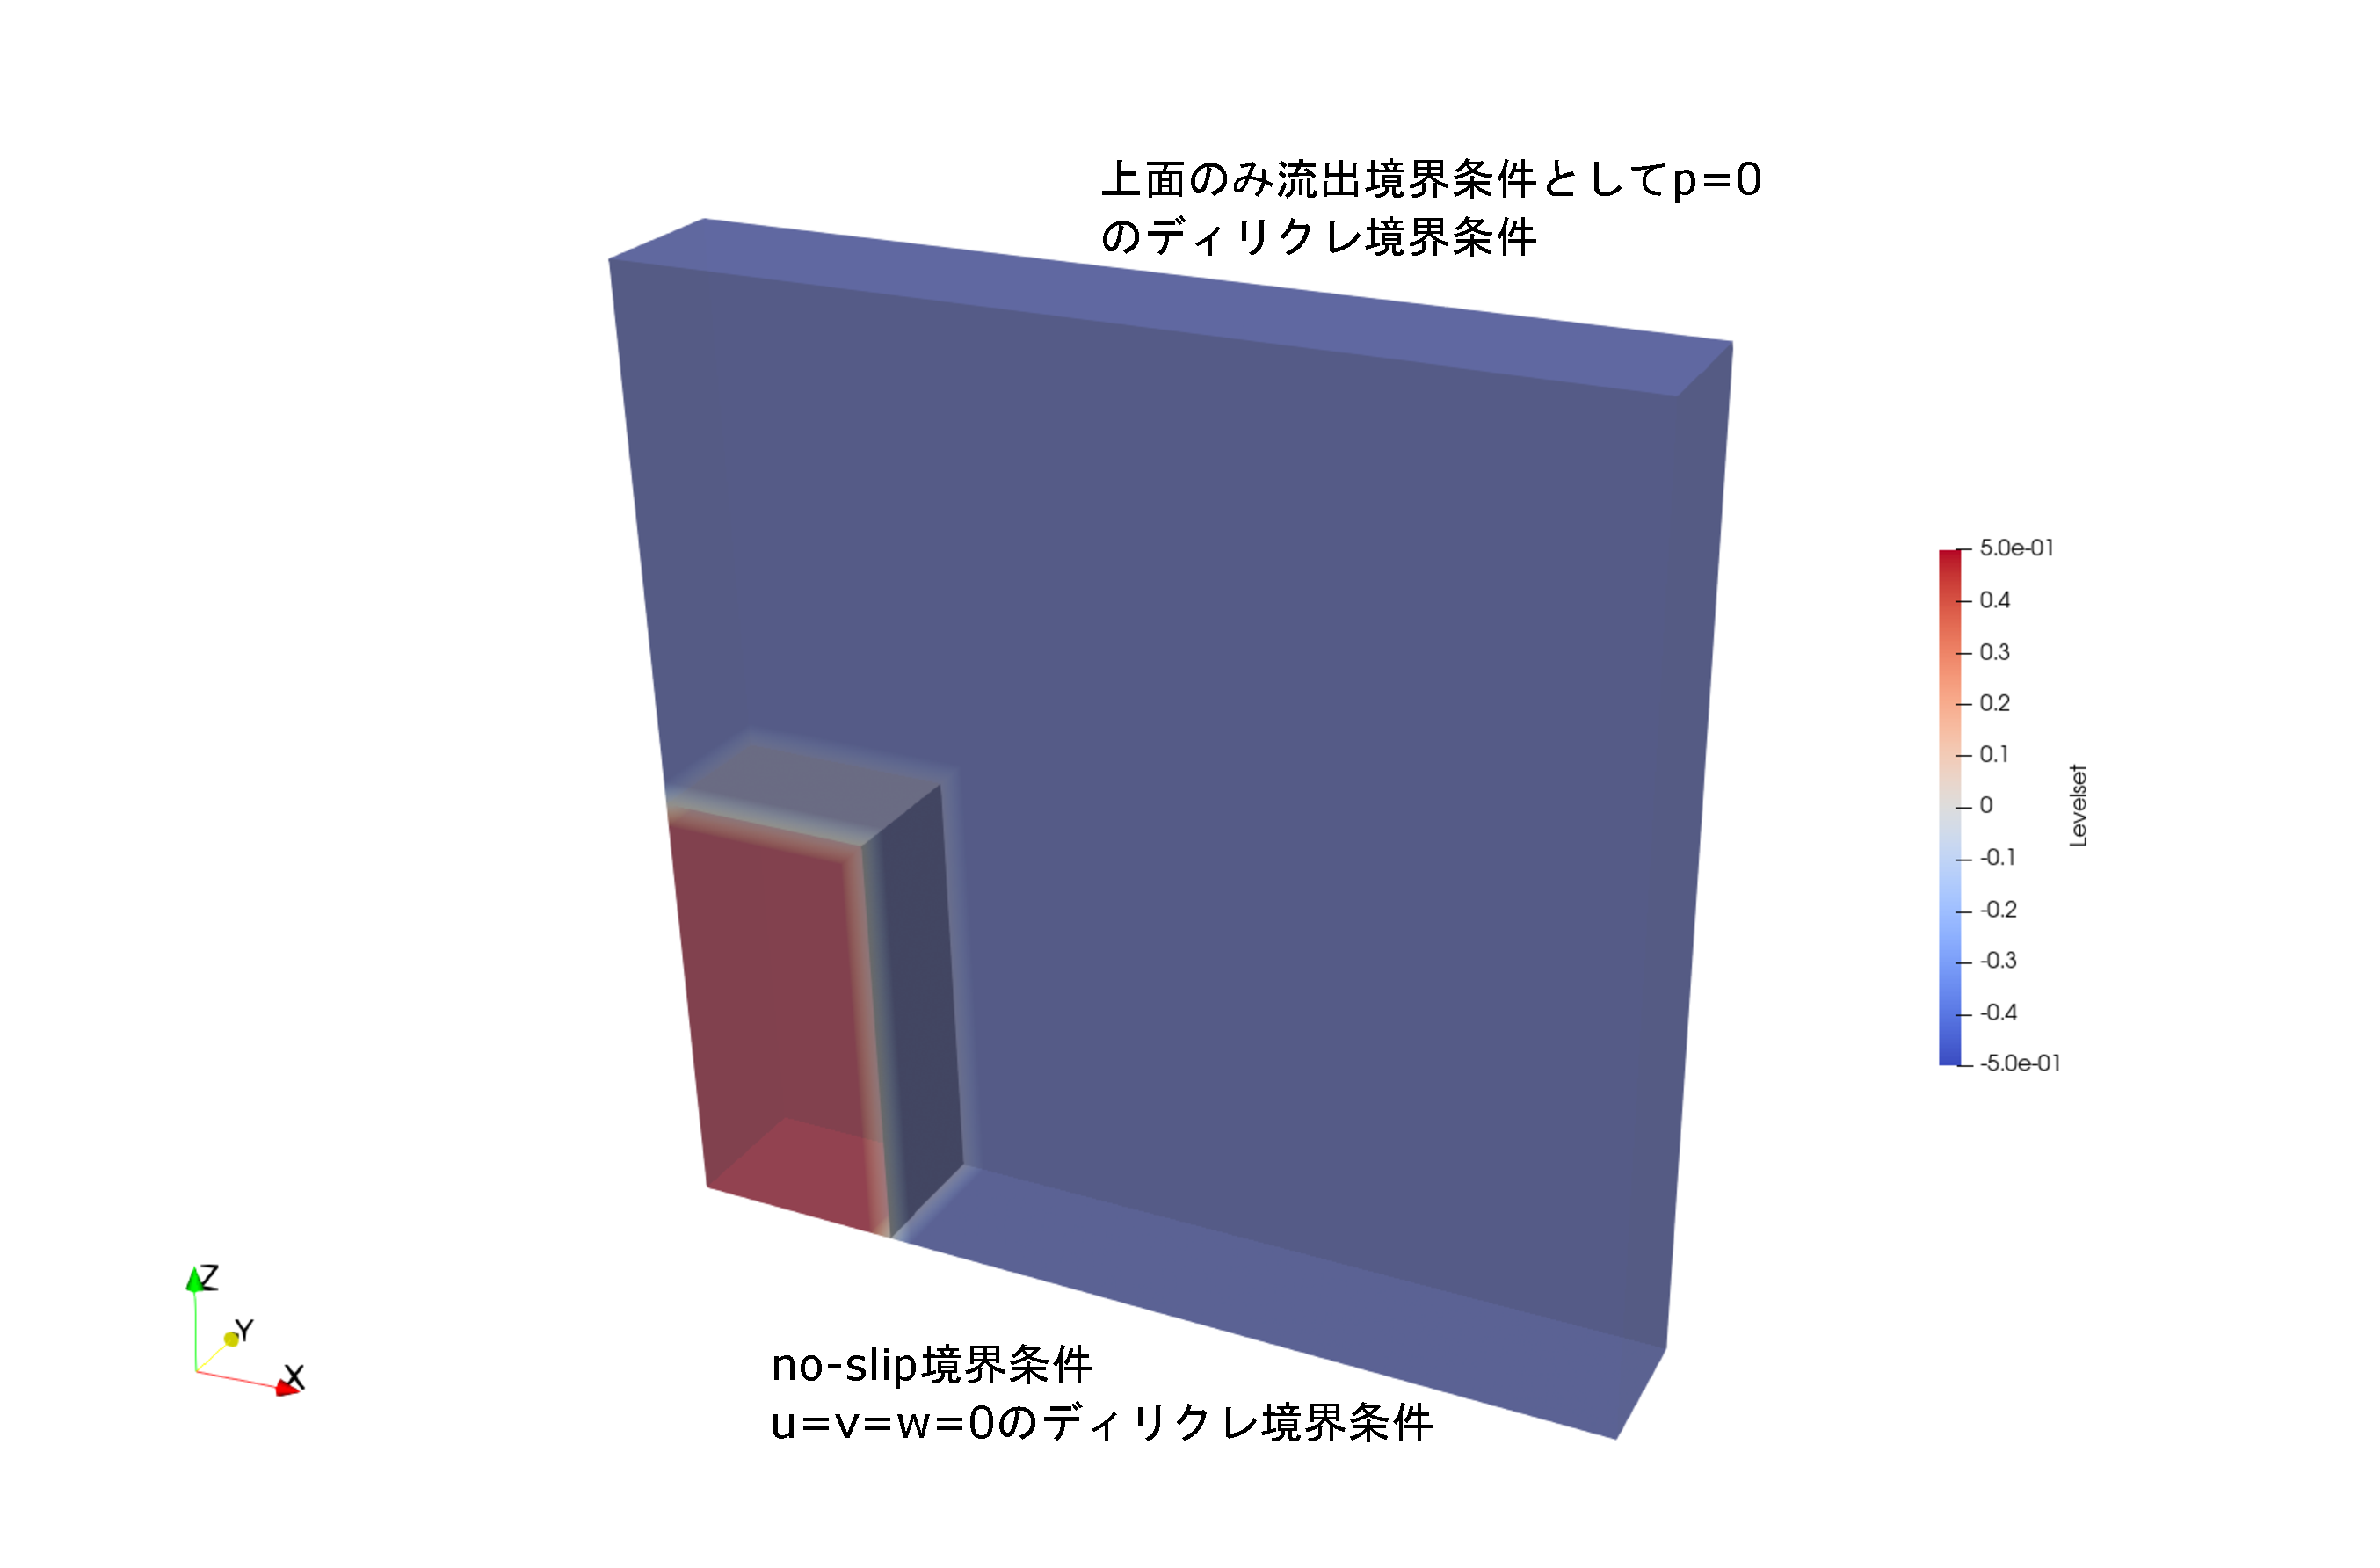
\includegraphics[width=6truecm]{pics/3d-sloshing/levelset_init.jpeg}
		\caption{3次元スロッシングのレベルセット関数($T=0$)}
		\label{fig:3d-sloshing-levelset_t0_3d}
	\end{minipage}
\end{figure}

\subsection{解析結果}
\subsubsection{メッシュ固定の場合の解析結果}
\begin{figure}[H]
    \centering
	\includegraphics[width=15truecm]{pics/3d-sloshing/height_time.pdf}
	\caption{スロッシング解析結果の左端の水位と参考文献\cite{Okamoto1992}, \cite{Sakuraba2001}との比較}
	\label{fig:3d-sloshing-result}
\end{figure}

\subsubsection{メッシュを移動させた場合の解析結果}
ここでは、メッシュを移動させた場合の結果を示す。

\subsubsection{並列化解析結果}
並列化させた場合の結果と計算時間の比較を示す。

